\section{进程相似性分析}

使用\perflow{}实现进程相似性分析的分析任务,在NPB基准测试程序和SWEEP3D上进行测试。测试结果如下:

\begin{figure}[!htb]
  \centering
  % \includegraphics[width=0.9\textwidth]{}
  \subfigure[BT]{
    \centering
    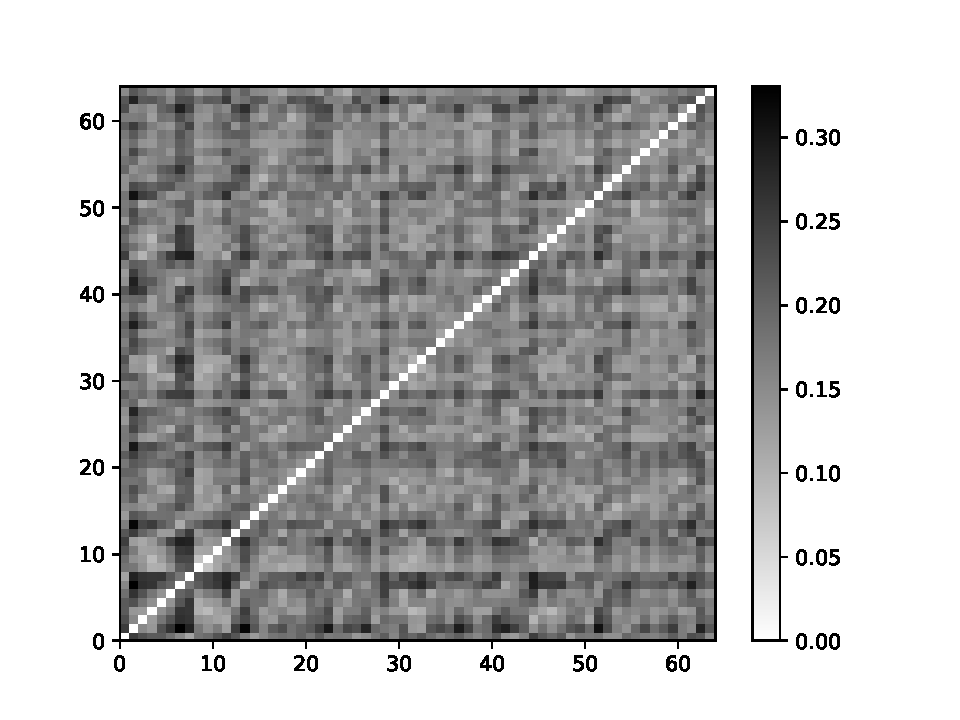
\includegraphics[width=0.3\textwidth]{procs_similarity/bt.B.pdf}
  }
  \subfigure[CG]{
    \centering
    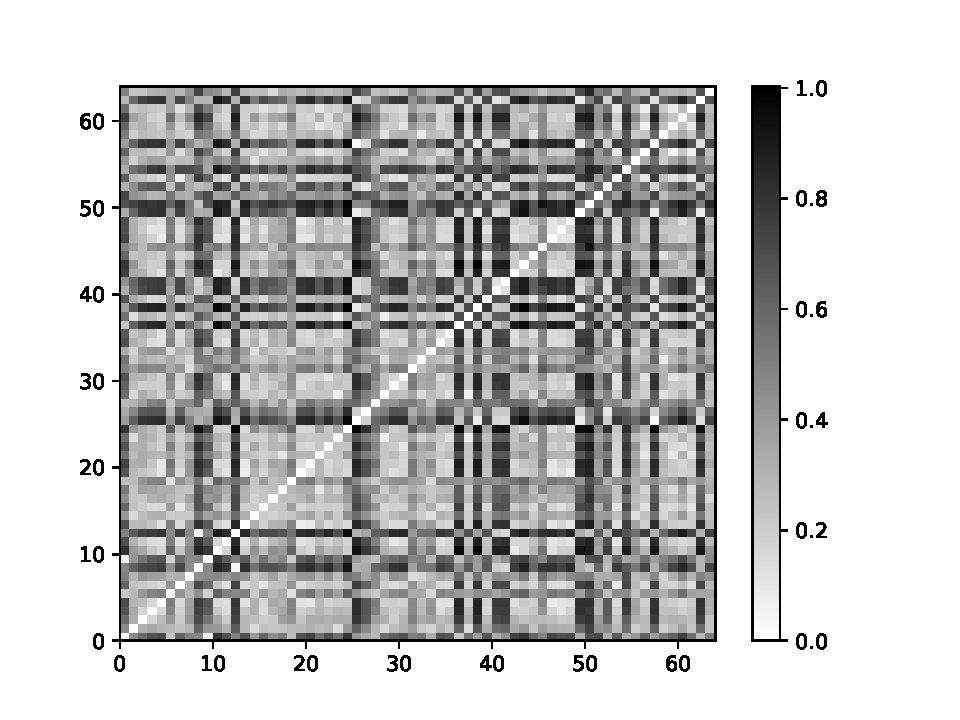
\includegraphics[width=0.3\textwidth]{procs_similarity/cg.B.pdf}
  }
  \subfigure[DT]{
    \centering
    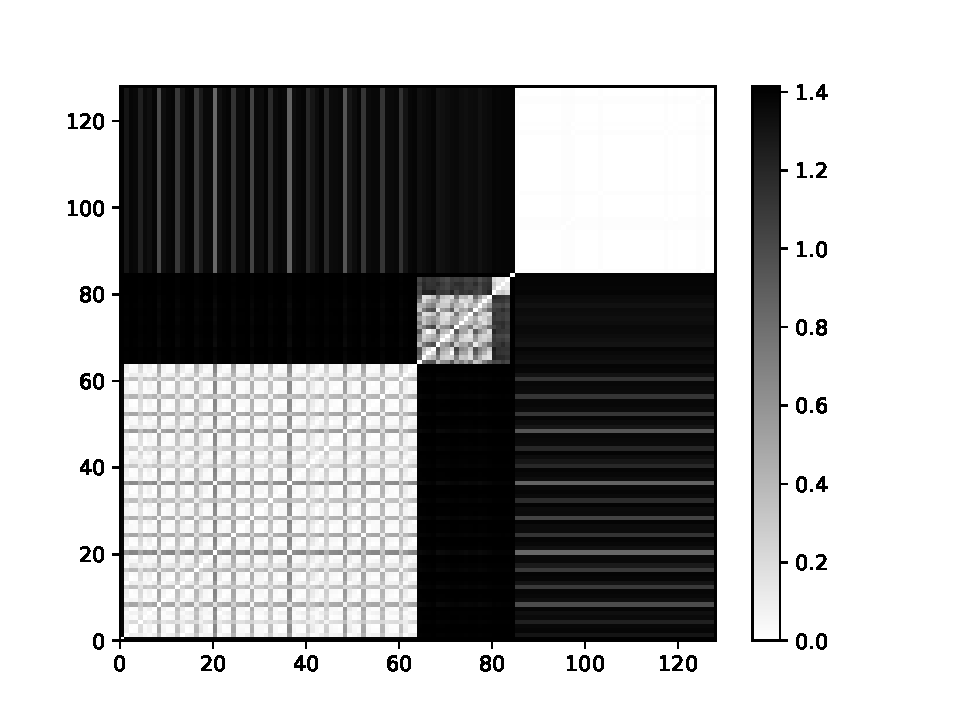
\includegraphics[width=0.3\textwidth]{procs_similarity/dt.C.pdf}
  }
  \subfigure[EP]{
    \centering
    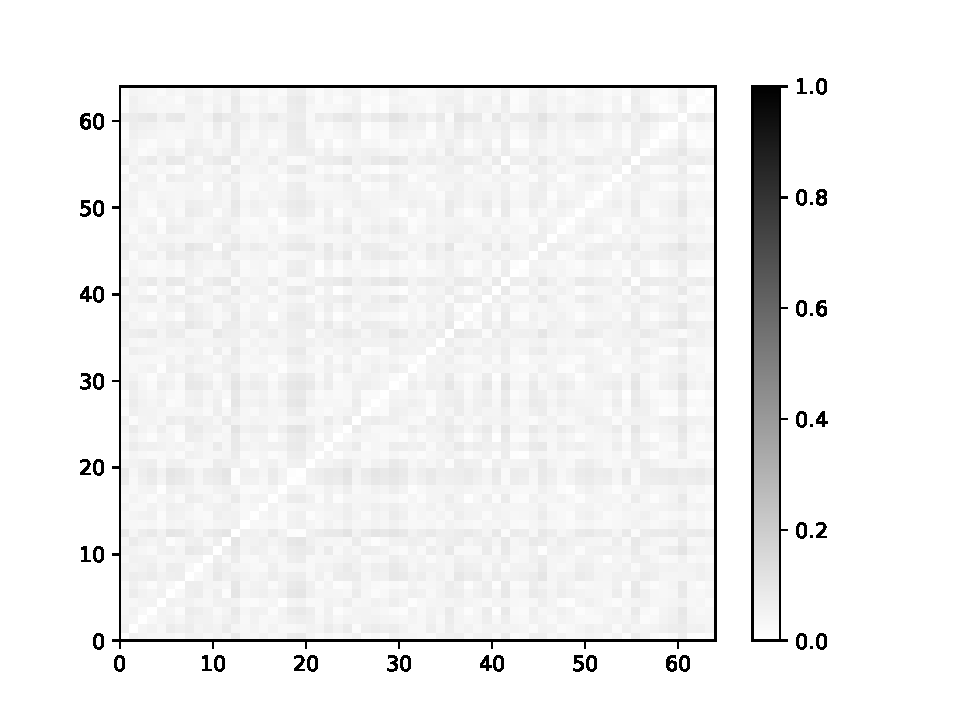
\includegraphics[width=0.3\textwidth]{procs_similarity/ep.C.pdf}
  }
  \subfigure[FT]{
    \centering
    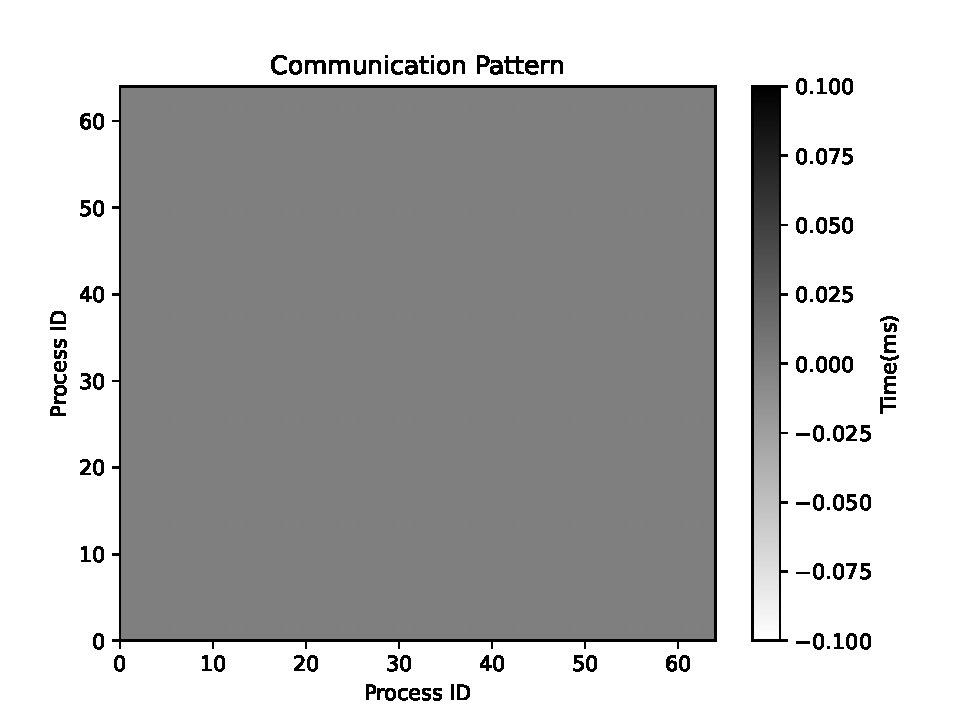
\includegraphics[width=0.3\textwidth]{procs_similarity/ft.B.pdf}
  }
  \subfigure[IS]{
    \centering
    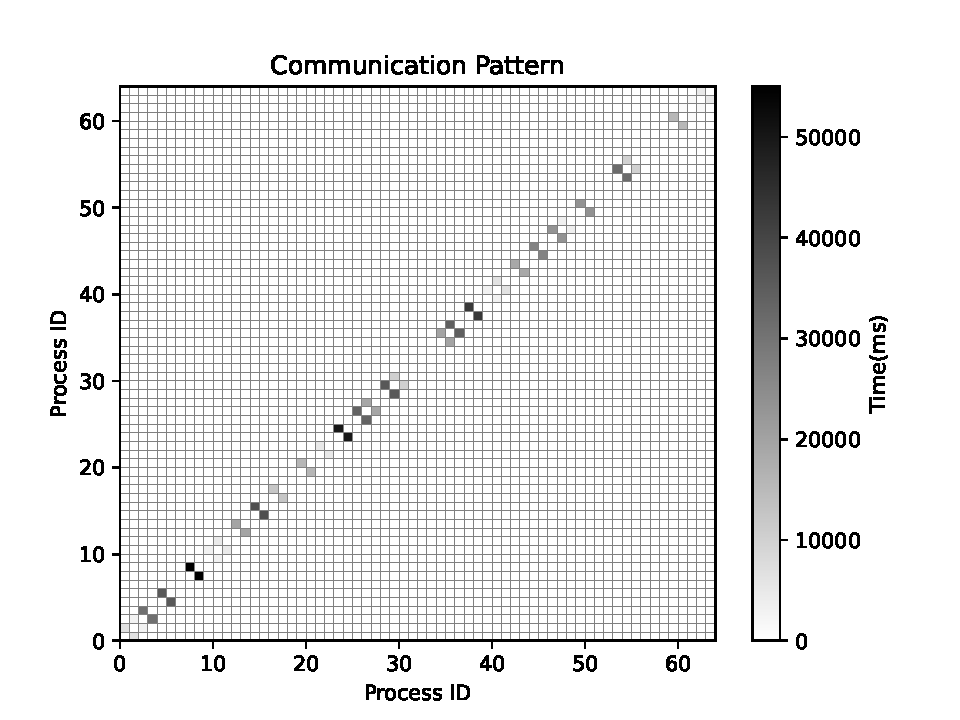
\includegraphics[width=0.3\textwidth]{procs_similarity/is.C.pdf}
  }
  \subfigure[LU]{
    \centering
    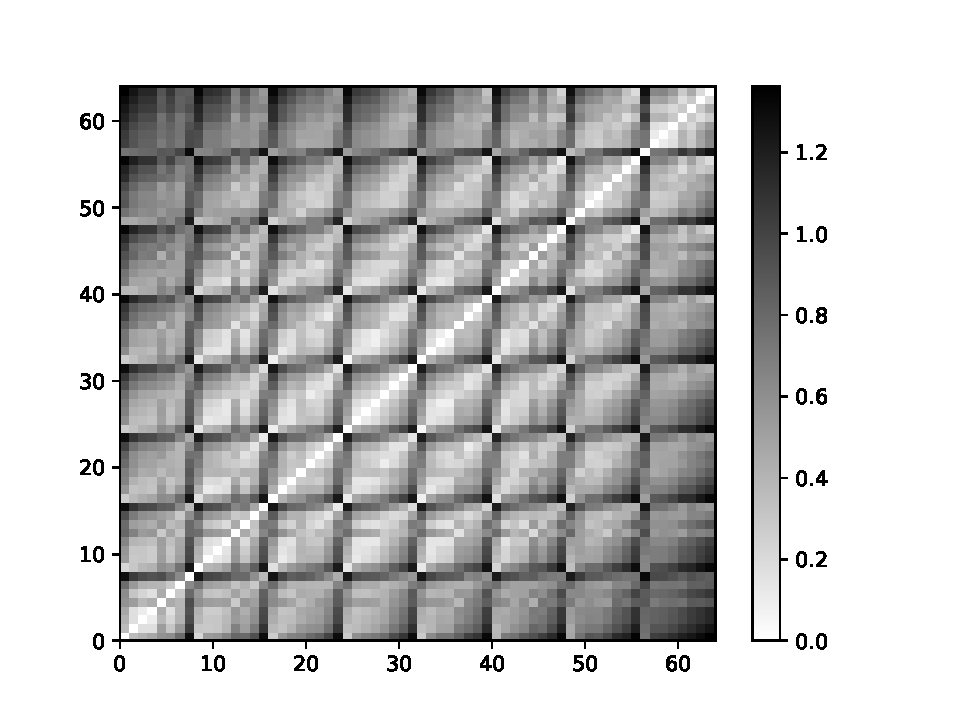
\includegraphics[width=0.3\textwidth]{procs_similarity/lu.B.pdf}
  }
  \subfigure[SP]{
    \centering
    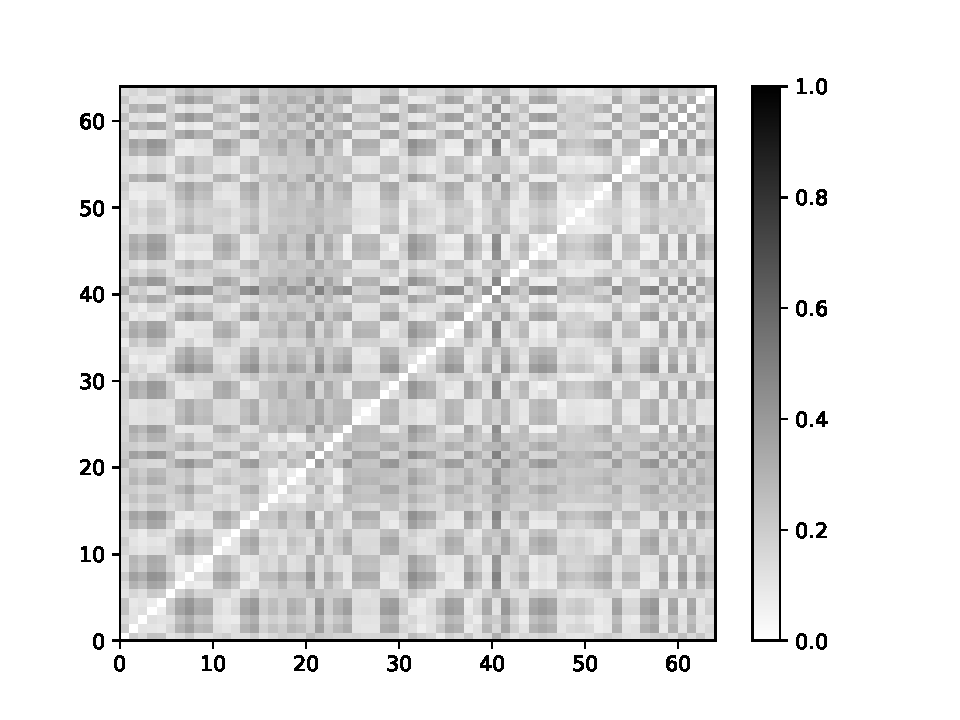
\includegraphics[width=0.3\textwidth]{procs_similarity/sp.B.pdf}
  }
  \subfigure[SWEEP3D]{
    \centering
    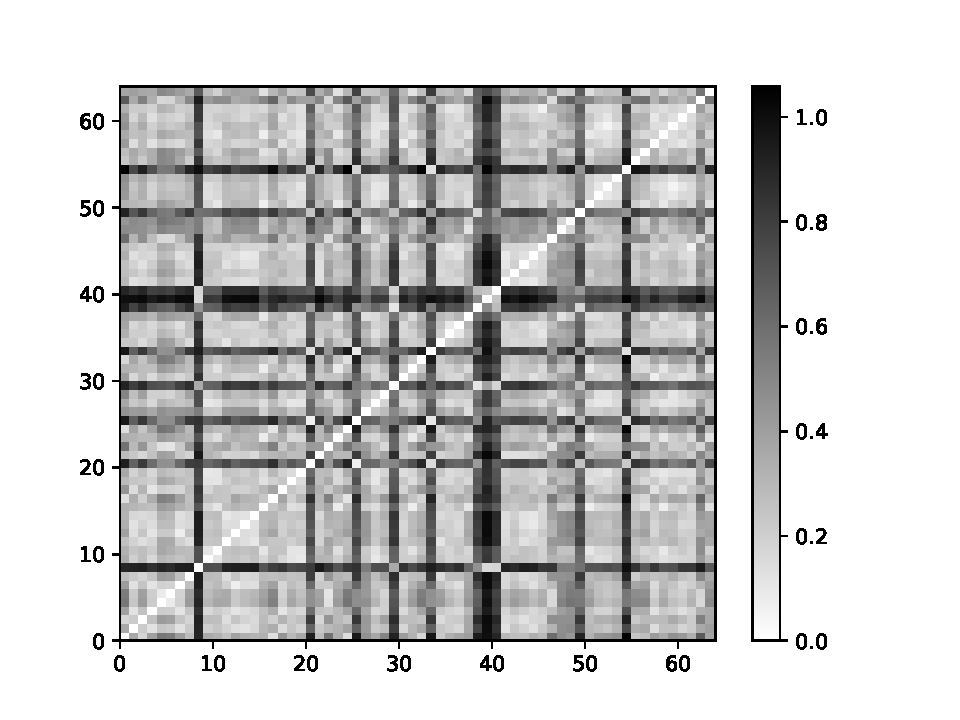
\includegraphics[width=0.3\textwidth]{procs_similarity/sweep3d.pdf}
  }
\end{figure}
